% \documentclass[review]{elsarticle}
\documentclass[utf8, babel, sor, jor, amsmath,amssymb, reprint]{elsarticle} %удалить перед отправкой
\usepackage[T2A]{fontenc} %удалить перед отправкой
\usepackage[utf8x]{inputenc} %удалить перед отправкой
\usepackage[english,russian]{babel} %удалить перед отправкой
\graphicspath{{images/}}

\usepackage{lineno,hyperref}
\usepackage{algorithm}
\usepackage{algorithmic}
\modulolinenumbers[5]

\journal{Journal of \LaTeX\ Templates}

%%%%%%%%%%%%%%%%%%%%%%%
%% Elsevier bibliography styles
%%%%%%%%%%%%%%%%%%%%%%%
%% To change the style, put a % in front of the second line of the current style and
%% remove the % from the second line of the style you would like to use.
%%%%%%%%%%%%%%%%%%%%%%%

%% Numbered
%\bibliographystyle{model1-num-names}

%% Numbered without titles
%\bibliographystyle{model1a-num-names}

%% Harvard
%\bibliographystyle{model2-names.bst}\biboptions{authoryear}

%% Vancouver numbered
%\usepackage{numcompress}\bibliographystyle{model3-num-names}

%% Vancouver name/year
%\usepackage{numcompress}\bibliographystyle{model4-names}\biboptions{authoryear}

%% APA style
%\bibliographystyle{model5-names}\biboptions{authoryear}

%% AMA style
%\usepackage{numcompress}\bibliographystyle{model6-num-names}

%% `Elsevier LaTeX' style
\bibliographystyle{elsarticle-num}
%%%%%%%%%%%%%%%%%%%%%%%


\usepackage{xcolor}
\newcommand{\todo}[1] {\textcolor{red}{#1}} %%for TODO comments
\def\l{\left\langle}
\def\r{\right\rangle}

\usepackage{mathrsfs}
\usepackage{amsmath}
\usepackage{amssymb}%



\begin{document}

\begin{frontmatter}


\title{Ground state search 2D Ising model}

\author[mainaddress, secondaryaddress]{Viacheslav Trukhin\corref{mycorrespondingauthor}}
\ead{trukhin.vo@dvfu.ru}

\author[mainaddress]{Egor Prokhorov\corref{mycorrespondingauthor}}
\ead{prokhorov.ei@dvfu.ru}

\author[mainaddress, secondaryaddress]{Konstantin Nefedev\corref{mycorrespondingauthor}}
\ead{nefedev.kv@dvfu.ru}


\address[mainaddress]{Far Eastern Federal University, Vladivostok, Russky Island, 10 Ajax Bay, 690922, the Russian Federation}
\address[secondaryaddress]{Institute of Applied Mathematics, Far Eastern Branch, Russian Academy of Science, Vladivostok, Radio 7, 690041, the Russian Federation}

\begin{abstract}


\end{abstract}


\begin{keyword}
Ising model, GPU and CPU high performance calculations, spin ice, spin glass, statistical thermodynamics.

\end{keyword}


\end{frontmatter}

\linenumbers
\newpage
\tableofcontents

\newpage
\section{Введение}



\section{Решение исчерпывающим перебором}

Модель спинового стекла Эдвардса-Андерсена представляет собой плоскую решетку Изинга:

\begin{equation}
	E = -\sum J_{ij} S_i S_j
	\label{eq:ising_energy}
\end{equation}

, где обменные интегралы $J$ могут принимать значения +1 или -1 создавая таким образом приближение аморфных материалов

Для решения такой цепочки из трёх спинов статистическая сумма
принимает вид:

\begin{equation}
	Z = e^{3\beta - 3\beta h} + 3e^{\beta - h - \beta} + 3e^{\beta h - \beta} + e^{3\beta + 3\beta h}
	\label{eq:stat_3}
\end{equation}

\section{Решение методом декомпозиции}

Рассматривая разные квадратные решётки из четырёх спинов взаимодействующих лишь с ближайшими соседями, можно заметить, что фрустрация в основном состоянии обязательно появляется, если в системе три обменных интеграла одного знака, а четвёртый другого.

\begin{figure}[h]
	\centering
	\resizebox{120px}{60px}{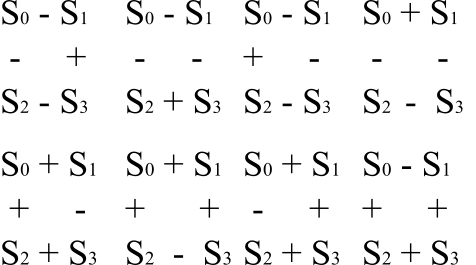
\includegraphics{2x2.1.png}}
	\caption{Фрустрированные квадратные системы}
	\label{fig:label}
\end{figure}

Полная энергия таких систем в соответствии с формулой \eqref{eq:ising_energy} принимает вид:

\begin{equation}
	E = -J_{01} S_0 S_1-J_{02} S_0 S_2-J_{13} S_1 S_3-J_{23} S_2 S_3.
	\label{eq:ising_energy_2x2}
\end{equation}

Поиск основного состояния данных систем методом полного перебора показывает, что каждая из этих систем имеет 8 основных состояний. Таким образом в основном состоянии каждая из пар спинов может быть фрустрирована.

Тогда логично предположить, что если система состоит из двух таких подсистем, то для минимизации энергии фрустрированная пара должна быть расположена на пересечении этих подсистем.
На Рис.2 пример решётки, состоящей из двух квадратных фрустрированных подсистем. Фрустрированной парой спинов будет пара $S_1$,$S_4$.

\begin{figure}[h]
	\centering
	\resizebox{75px}{55px}{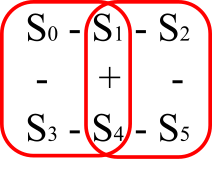
\includegraphics{3x2.png}}
	\caption{Решётка,состоящая из двух квадратных фрустрированных подсистем}
	\label{fig:label}
\end{figure}


Метод полного перебора подтверждает правильность данного решения. В Таблице 1 приведены низкоэнергетические состояния данной решётки, полученные с помощью полного перебора состояний. Конфигурации спинов в основных состояниях доказывают что фрустрированной парой является пара $S_1$,$S_4$

\begin{table}[h]
	\centering
	\begin{tabular}{|c|c|}
		\hline
		 E   &   Конфигурация спинов \\
		 \hline
		-5   &   -1-1-1-1-1-1 \\
		\hline
		-3   &  -11-1-1-1-1 \\
		\hline
		-3   &   11-1-1-1-1 \\
		\hline
		-3   &   -111-1-1-1 \\
		\hline
		-3   &   111-1-1-1 \\
		\hline
		-3   &   11-11-1-1 \\
		\hline
		-3   &   1111-1-1 \\
		\hline
		-3   &   -1-1-1-11-1 \\
		\hline
		-3   &   -1-1-111-1 \\
		\hline
		-3   &   1-1-111-1 \\
		\hline
		-3   &   -111-1-11 \\
		\hline
		-3   &   111-1-11 \\
		\hline
		-3   &   1111-11 \\
		\hline
		-3   &   -1-1-1-111 \\
		\hline
		-3   &   -1-11-111 \\
		\hline
		-3   &   -1-1-1111 \\
		\hline
		-3   &   1-1-1111 \\
		\hline
		-3   &   -1-11111 \\
		\hline
		-3   &   1-11111 \\
		\hline
		-5   &   111111 \\
		\hline
	\end{tabular}
	\caption{Низкоэнергетические состояния решётки}
	\label{tab:table_low_energy}
\end{table}

Таким образом, зная где расположена фрустрированная пара спинов, а следовательно, и где расположены не фрустрированные пары, можно найти основное состояние системы просто расставляя значение спинов по порядку или с начиная с любого спина. Полученная данным методом конфигурация и значение энергии также соответствуют основному состояния приведнном в Таблице \eqref{tab:table_low_energy}.

Если рассматриваемые квадратные фрустрированные решётки пересекаются с несколькими себе подобными, то они формируют кластер.

\begin{figure}[h]
	\centering
	\resizebox{140px}{50px}{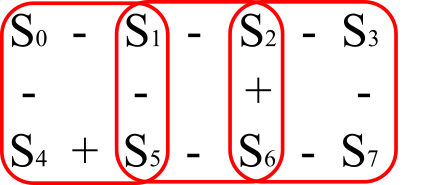
\includegraphics{4x2.png}}
	\caption{Кластер фрустрированных квадратных решёток}
	\label{fig:cluster}
\end{figure}

В кластере необходимо выбрать фрустрированными пары, находящиеся на пересечении так чтобы такая пара была в подсистеме только одна. Если в каком-то состоянии подсистема осталась без выбранной пары в силу невозможности её расположения на пересечении подсистем, выбирается одна из трёх оставшихся в подсистеме пар, по возможности та, которая не будет возбуждать другие подсистемы, не входящие в кластер .Это можно сделать с помощью полного перебора состояний пар, где состояние пары может принимать только два значения: пара фрустрирована и пара не фрустрирована.

В данной системе \ref{fig:cluster} можно выбрать фрустрированной пару $S_1$,$S_5$, тогда пару  $S_2$,$S_6$ выбрать уже нельзя. Второй фрустрированной парой можно выбрать оду из трёх оставшихся в подсистеме пар: $S_2$ $S_3$, $S_3$,$S_7$ или $S_6$,$S_7$. Если изначально выбирается пара $S_2$ $S_6$, то второй будет пара $S_0$ $S_1$, $S_0$,$S_4$ или $S_4$,$S_5$. Далее для каждой из конфигураций фрустраций в системе расставляются значения спинов. Таким образом для данной системы получается 12 основных состояний.

Полный перебор состояний данной системы подтверждает правильность расстановки фрустраций в решётке, энергию и кратность вырождения.

\begin{table}[h]
	\centering
	\begin{tabular}{|c|c|}
		\hline
		E   &   Конфигурация спинов \\
	\hline
	-6      &       -1-1-1-1-1-1-1-1 \\
	\hline
	-6      &       -1-1-1-11-1-1-1 \\
	\hline
	-6      &       1-1-1-11-1-1-1  \\
	\hline
	-6      &       111-11-1-1-1    \\
	\hline
	-6      &       11111-1-1-1     \\
	\hline
	-6      &       -1-1-1-1-111-1  \\
	\hline
	-6      &       11111-1-11      \\
	\hline
	-6      &       -1-1-1-1-1111   \\
	\hline
	-6      &       -1-1-11-1111    \\
	\hline
	-6      &       -1111-1111      \\
	\hline
	-6      &       1111-1111       \\
	\hline
	-6      &       11111111        \\
	\hline
	\end{tabular}
	\caption{Основные состояния кластера}
	\label{tab:table_low_energy_4x2}
\end{table}

\begin{figure}[h]
	\centering
	\resizebox{310px}{220px}{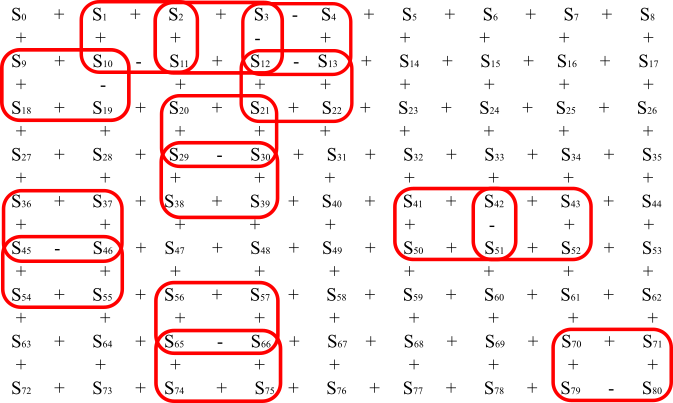
\includegraphics{9x9.png}}
	\caption{Квадратная решётка из 81 спина}
	\label{fig:label_9x9}
\end{figure}

Определить основные состояния можно и на решётках больших размеров \ref{fig:label_9x9}, применяя все те же самые рассуждения. Энергия основного состояния, его кратность вырождения и спиновый избыток также совпадает с решением исчерпывающим перебором.

\begin{figure}[h]
	\centering
	\resizebox{310px}{220px}{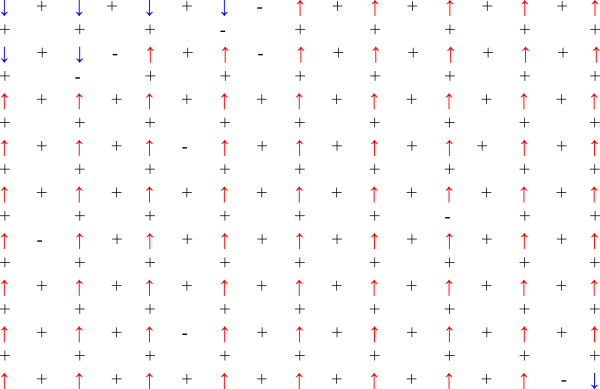
\includegraphics{9x9_gs_1.png}}
	\caption{Одно из основных состояний решётки \eqref{fig:label_9x9}}
	\label{fig:label_9x9_gs_1}
\end{figure}

\section{Благодарности}

 

\bibliography{mybibfile}


\end{document}